\documentclass{article}
\usepackage{natbib}
\usepackage{amsmath,amssymb,amsfonts}
\usepackage[table]{xcolor}
\usepackage{url}
\def\UrlBreaks{\do\/\do-}
\usepackage{float}
\pdfminorversion=4
\usepackage[letterpaper,top=2cm,bottom=2cm,left=3cm,right=3cm,marginparwidth=1.75cm]{geometry}
\usepackage{algorithm}
\usepackage{algpseudocode}
% Useful packages
\usepackage{graphicx}
\graphicspath{{Images/}}
\usepackage[colorlinks=true, allcolors=blue]{hyperref}

\usepackage{adjustbox}
\usepackage{array,multirow}
\usepackage{booktabs}
\usepackage{nicematrix}
\usepackage{caption}
\usepackage{subcaption}

\usepackage{blindtext}
\usepackage{titlesec}
\usepackage{natbib}
\title{Effect of prior knowledge in missing person search and its use in human swarm interaction strategies}
%\date{September 2023}

\begin{document}

\maketitle

\section{Introduction}
 Between 1992 and 2007, there were a total of 65,439 missing person incidents in the National Parks in United States \cite{heggie2009dead}. Most of these incidents occur in National Parks.  In 2005, only five national parks accounted for close to fifty percent of such incidents. Without an effective search and rescue (SAR) response, one in five such incidents would result in a fatality \cite{heggie2009dead}. 

In wilderness search and rescue, one of the first steps is to establish a point last seen (PLS) or last known point (LKP), depending on where the missing person was last sighted or where they were last assumed to be. Once a PLS is known, search areas are established by analyzing lost person behavior and terrain. The search areas are then prioritized based on metrics such as probability of area (POA), which is the probability that the lost person is contained within a particular region \cite{doherty2014analysis}. Actual search often involves rescuers who use small aircrafts to systematically search within the POAs. Because the search area grows geometrically with time, locating a lost person alive is a time critical task. 

Conventional SAR operations involve teams of searchers on the ground coordinating with central operations relying on the ground searchers skill and knowledge of the area, or search in grids where searchers form a line facilitating wide area search or using dogs who track the missing person down by scent \cite{dickSAR}. Rescuers also use small aircraft and helicopters equipped with thermal cameras to sweep large areas and located missing persons, additionally hard to reach areas can be accessed relatively easily from air \cite{dickSAR}. Over the past decade, unmanned aerial vehicles (UAV) are being increasingly used in search and rescue (SAR) missions to find missing persons \cite{tusnio2021efficiency,goodrich2008supporting,grogan2018use}. While completely autonomous solutions that enable terrain following \cite{silvagni2017multipurpose} and swarm based solutions that cover large areas \cite{nunnally2012human} are part of ongoing research, a common use of UAVs in SAR involves searching by teleoperation with a live camera feed \cite{delmerico2019current, isaacs2022teleoperation}. %In recent years, unmanned aerial vehicles (UAVs) equipped with cameras have been used in SAR missions especially those that are conducted in harsh terrains \cite{yong2018human}.


A SAR mission with teleoperated UAVs involves skilled operators who are expected to search efficiently within a region that has a high probability of finding the missing person. In doing so, the operators are presumed to take into account missing person behavior and terrain features \cite{niedzielski2018real, koester2008lost}. In reality however, teleoperators may not be familiar with the terrain they are flying over \cite{burke2004moonlight} or fully understand the behavior profile of the missing person in terms of how fast they may be going, their mental state, or whether they will stay near the trails \cite{syrotuck2000}. Thus, prior knowledge, not skill, can be an important factor in search performance. Indeed, as has been shown in missing person models, such prior knowledge about the missing person and the terrain can significantly affect mission performance by improving the accuracy of search regions \cite{lin2010bayesian,hashimoto2022agent}.
	
In this context, a better understanding of how prior knowledge affects teleoperator actions can enable prior knowledge inference from UAV movement in the field. In a human-swarm interaction (HSI) setup where the operator interacts directly with the swarm on the field \cite{kolling2015human}, such inference can be used to control other autonomous robots in the field, who may then utilize adaptive control strategies to selectively search near or far from teleoperators \cite{krzysiak2021information}. Such strategies could additionally account for the cognitive load on the teleoperator and regulate their actions accordingly such as providing assistance only when the operator is experiencing low cognitive load. In light of limited bandwidth in swarm robot settings, such prior knowledge inference and cognitive load inference would be best obtained through non-verbal movement cues observed directly on the field. At the same time, understanding how teleoperators perceive presence of other robots on the field may aid in providing nonverbal cues towards where to search \cite{st2019collective, santos2021motions}. 
	%From a user-interface design perspective, the effect of prior knowledge on mental workload, can be used to provide custom cues on the heads-up-displays of the teleoperators improving their efficiency \cite{anderson2021user}.

Accordingly, this work is motivated by the following hypotheses. For a teleoperator searching for a missing person, the movement cues of the teleoperated UAV are: (H1)  affected by prior knowledge of terrain or missing person and (H2) by the cognitive load of a teleoperator. The results of these hypotheses are then used to motivate the design of an LSTM algorithm to directly infer prior knowledge and cognitive load from movement data available in the field. Results from these hypotheses were then used to design a new robot control strategy that exploits prior knowledge. Specifically, in this strategy multiple robots infer and act on prior knowledge regulated by cognitive load. This strategy is then compared to other approaches where multiple robots in a swarm search in random locations independently, follow the human teleoperator, or search in a spiral pattern.  


Accordingly, in this study, we first conduct an experimental study to test hypotheses related to the effect of prior knowledge and cognitive load on search behavior. The study is conducted on virtual 10 $\times$ 10 km replica of a section of the Grand Canyon National Park, which reports one of the largest number of missing person cases every year. Participants were briefed with prior knowledge about the local terrain and the missing person before every trial. To study the effect of perception of other UAVs in the environment, we placed UAVs in random locations as a cluster (to indicate the possibility useful information in the region \cite{st2019collective}) or spread them out within the environment. Participant EEG is recorded during experiments  measure cognitive load experienced. Because EEG data is prone to noise from movement we additionally use an eye tracker to investigate if pupil dilation correlates with cognitive load in such scenarios. Next, we validate a long-short-term memory (LSTM) model to infer the presence of prior knowledge based on limited observation of the trajectory data of a teleoperated drone. Finally, we formulate and compare a robot swarm control strategy that adapts its search behavior in response to prior knowledge inference and cognitive load by simulating the swarm to respond to experimental data of human teleoperation during search.
	
%To create prior knowledge, we selectively reveal aspects of the environment and the missing person to participants before they search through the park for the missing person. 

%Our analyses reveal dependencies of performance, behavior, attention, and cognitive load on the presence of prior knowledge and swarm distribution. 


%This work is motivated by the following research questions: (i) does prior knowledge of terrain or missing person affect teleoperator search performance and actions? (ii) does prior knowledge affect mental workload and gaze behavior? (ii) can the existence of such prior knowledge be inferred using data-driven methods? and (iv) how does a control strategy where multiple robots infer and act on prior knowledge in the field compare to strategies where multiple robots in a swarm search randomly or follow the human teleoperator? 

This paper is organized as follows: section \ref{sec:exptMethod} describes the experimental methods including the modeling of the virtual environment, gaze and electroencephalography (EEG) setup, experimental setup and procedure and, experimental results. Section \ref{sec:LSTM} presents a machine learning algorithm for human prior knowledge classification, and optimal parameter selection. Section \ref{sec:controlStrategy} simulation conditions and setup, control strategy of robot swarm, and simulation results. Section \ref{sec:discussion} concludes with a discussion of the results and applications of this work.


\section{Related work}

Teleoperating a single UAV with possible assistance from autonomous UAVs is a common mode for search and rescue operations. While purely autonomous  solutions are increasingly proposed in the literature, the level of risk associated with missing person search, makes human involvement for detection and rescue inevitable. A SAR mission that utilizes teleoperated UAVs is expected to involve skilled tele-operators who may not be familiar with the local terrain \cite{}. Furthermore, information about the missing person themselves may be interpreted and integrated differently into search strategies by each teleoperator \cite{}. Interviews with SAR responders in regions with extreme climates regarding the use of UAVs have highlighted the need to assimilate vasts amounts of additional information including environmental conditions and legal restrictions in addition to dealing with local capacities \cite{Clark2018}. 

In this context, assistance to the teleoperator may be provided in the form of interface design which enables improved search regions \cite{Nourbakhsh2005, Goodrich2007using, heintzman2021predictive} and situational awareness\cite{Riley2004}, coordinated efforts between ground and aerial searchers \cite{niedzielski2018real}, shared autonomy \cite{wegner2006agent}, where an intelligent UAV may selectively ignore or blend human control input with its own inference of the mission, or multiple autonomous UAVs may intelligently search the region to minimize search time \cite{hardin2009using}. 

Specifically, humans may be involved in base operations receiving critical information periodically from UAVs that can be integrated with lost person behavior simulations to take search decisions \cite{Nourbakhsh2005, Goodrich2007using}. More recently, a long-short-term memory (LSTM) network has been used to predict human actions that are integrated into a game theoretic model to act as a decision aid to plan search and compute lost person trajectories \cite{heintzman2021predictive}. As teleoperators that see remote locations from a local interface, Riley et al. have highlighted the role of interface design and team formation towards attaining attain situational awareness in SAR missions \cite{Riley2004}. Niedzielski et al. demonstrate the effectiveness of a coordinated search and rescue strategy where teleoperators search POAs as they are assisted by imagery analysts to identify the missing person, who is then rescued by ground searchers \cite{niedzielski2018real}. The POAs on the map are drawn based on a lost-person mobility model that takes into account the terrain features to delineate areas of easy access by the missing person. 

Shared autonomy approaches include the use of blended autonomy, where a mediation agent blends command from the tele-operator with the autonomous actions of robots based on sensory input, in some cases an intervention from the tele-operator is required before progressing \cite{wegner2006agent}, adaptive autonomy \cite{hardin2009using} where the autonomous robots decide themselves which tasks to execute; adjustable autonomy, where the tele-operator assigns tasks to the robots, and mixed initiative, where the robots and tele-operator collaboratively decide the level of autonomy.  More recently, Krzysiak and Butail \cite{krzysiak2021information} provide a framework for blending mutual information instead of control inputs to provide a context independent search strategy for coordination between a teleoperator and autonomous robots. This study focuses on enabling a similar framework through the inference of prior knowledge AND COGNITIVE LOAD from non-verbal movement cues. The use of movement cues allows communication-free implementation of robotic swarm assistance in the field. 


% NEED MORE PAPERS ON HUMAN-ROBOT INTERACTION OR HUMAN-SWARM INTERACTION FOR SEARCH. Use the list below

% Goodrich, M. A., Cooper, J. L., Adams, J. A., Humphrey, C., Zeeman, R., & Buss, B. G. (2007, September). Using a mini-uav to support wilderness search and rescue: Practices for human-robot teaming. In 2007 IEEE International Workshop on Safety, Security and Rescue Robotics (pp. 1-6). IEEE.
% Nourbakhsh, I. R., Sycara, K., Koes, M., Yong, M., Lewis, M., & Burion, S. (2005). Human-robot teaming for search and rescue. IEEE Pervasive Computing, 4(1), 72-79.
% Riley, J. M., & Endsley, M. R. (2004, September). The hunt for situation awareness: Human-robot interaction in search and rescue. In Proceedings of the Human Factors and Ergonomics Society Annual Meeting (Vol. 48, No. 3, pp. 693-697). Sage CA: Los Angeles, CA: SAGE Publications.
%Clark, D. G., Ford, J. D., & Tabish, T. (2018). What role can unmanned aerial vehicles play in emergency response in the Arctic: A case study from Canada. PLoS One, 13(12), e0205299.


%Papaioannou et. al. propose a distributed search and planning framework where a dynamically varying team of autonomous robots cooperate to search for targets \cite{papaioannou2023distributed}. To maximize the effectiveness of an UAV swarm search team, Kashino et. al. optimize task allocation and trajectory planning using iso-probability curves in the continuous domain, wherein the UAVs traverse a range of iso-probability curves throughout the search \cite{kashino2020adaptive}. In situations where the missing person may have access to a transponder, UAVs can be used to localize a possibly non-static signal source by using time difference of arrival \cite{khalil2023uavs}. Similarly, Dinh et. al. propose a system of UAVs that are capable of detecting mobile phone signals by triangulating the signal source  \cite{dinh2019unmanned}. Heintzman et. al. set up a pre-planned trajectories for UAVs that can assist the searchers on the ground \cite{heintzman2021anticipatory}. The trajectories are created taking into account a predictive lost person model, topography of the environment, and anticipated ground crew trajectories.

\section{Background}
\subsection{Prior knowledge}
Prior knowledge refers to relevant information about the task at hand that could be retrieved to improve task efficiency. Prior knowledge has been shown to require additional cognitive capacity \cite{Britton1982}, ... [more effects of prior knowledge in other contexts]

Examples of prior knowledge in the context of SAR include lost person information or terrain knowledge. While such information may be provided to a skilled UAV operator prior to a mission, it may not be effectively utilized at all times. In a  SAR scenario, prior knowledge may be used to guide search actions such as searching within a particular region or near trails. At the same time, in the absence of a clear mental model, it is difficult to quantify whether prior knowledge is properly utilized by a teleoperator in their search \cite{Burke2004}. 


\subsection{Cognitive load}
Cognitive load is the mental workload experienced by a human as they perform a task \cite{Paas2003}. Cognitive load can be measured through survey responses \cite{Sweller2011}, secondary task performance \cite{Anderson2011}, electroencephalogram (EEG)  data \cite{many papers}, and pupillometry data \cite{more papers}.  During a complex time intensive task such as search and rescue cognitive load can play a critical role in modulating task performance \cite{?}. Specifically...
\subsection{Swarm perception}



\subsection{Distributed swarm control}


\section{Problem statement}
Consider a wilderness SAR scenario where a team of a single human teleoperated robot and a swarm of autonomous robots are searching for a missing person. Due to the large search area, the human teleoperator can only see the autonomous robot positions in an overhead view available in an inset on their feed. Compared to the human teleoperator, the autonomous robots have a lower detection rate of 0.66. 

We assume no communication between the teleoperator to the autonomous robots beyond the two types being aware of each other's location. This is because information about knowledge or cognitive state may create security vulnerabilities \cite{} and information from the autonomous robots to the teleoperator may pose additional cognitive burden. The goal of the mission is to find a missing person as soon as possible.
%\section{Swarm control in response to prior knowledge}


\section{Experimental study}
\subsection{Virtual Environment}
	\begin{figure}[ht!]
		\centering
		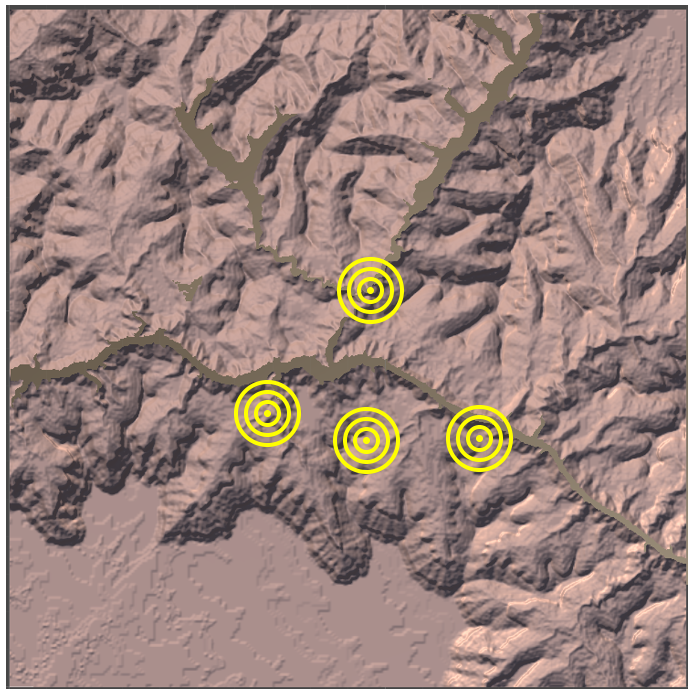
\includegraphics[width=0.99\linewidth]{images/grandCanyonTop_v2.png}
		\caption[width=0.99\linewidth]{An overhead view of the 10 km $\times$ 10 km virtual environment designed after the Grand Canyon National park using height map data. The four sets of concentric circles are centered at the four positions where the missing person could be last seen (PLS). One of these four locations was randomly selected for trials within the experiment. The size of the circles correspond to different distances from the PLS  based on how fast the missing person may have walked since they were last sighted.}
		\label{fig:grandCanyonTopView}
	\end{figure}
	
	The virtual environment consisted of a 10 km $\times$ 10 km replica of a section of the Grand Canyon National Park (fig. \ref{fig:grandCanyonTopView}). The park terrain was built in Unity software using height-map data obtained from an online heightmap generator \cite{heightmapsite}. The location of the terrain was approximately centered at coordinates 36$^{\circ}$5'57" N and 112$^{\circ}$5'38" W. The terrain was further enriched using trees and static water marking the Colorado River. The light brown color of the landscape was selected to match pictures of the park. 
	
	A virtual quadrotor UAV (quad-copter Simulation asset, Unity Assets) capable of flying in three dimensions was used to navigate the terrain. The operator could use arrow keys to move in front-back and left-right directions, and `r' and `f' keys to move up and down respectively. The UAV used realistic dynamics to simulate the motion while producing sound and rotor speeds in proportion to the thrust applied in each direction. 
	
	A camera fixed to the UAV provided the teleoperator a first person view (FPV) of the environment with UAV telemetry data superimposed on the display (fig. \ref{fig:HUDandMissingPerson}).  The camera could be pivoted to pitch up and down with `w' and `s' keys providing a front or downward facing view of the virtual environment. 
	
	The FPV display (fig. \ref{fig:HUDandMissingPerson}) also showed an overhead GPS map of the environment in an inset on top right. This inset showed the position where the missing person was last sighted (PLS), and three concentric rings marking the high probability regions called probability of areas (POAs) where the missing person may be found based on their walking speed. These were set at radii 0.36 km, 0.72 km, and 1.08 km corresponding to the average distance moved by a random walker at walking speeds of 1, 2, and 3 m/s respectively. The position of the teleoperated UAV was shown on the inset as a green circle with a yellow line pointing in the direction of heading. A swarm of 50 other UAVs were also placed in the environment and could be seen as red circles on the inset. 
	
	The missing person was modeled as a male individual who wore a t-shirt and shorts. To further improve visibility and detectability, an emergency flare was simulated near the missing person to send out red smoke that dissipated with distance. % 620 m 
	
	
	\begin{figure}[ht!]
		\centering
		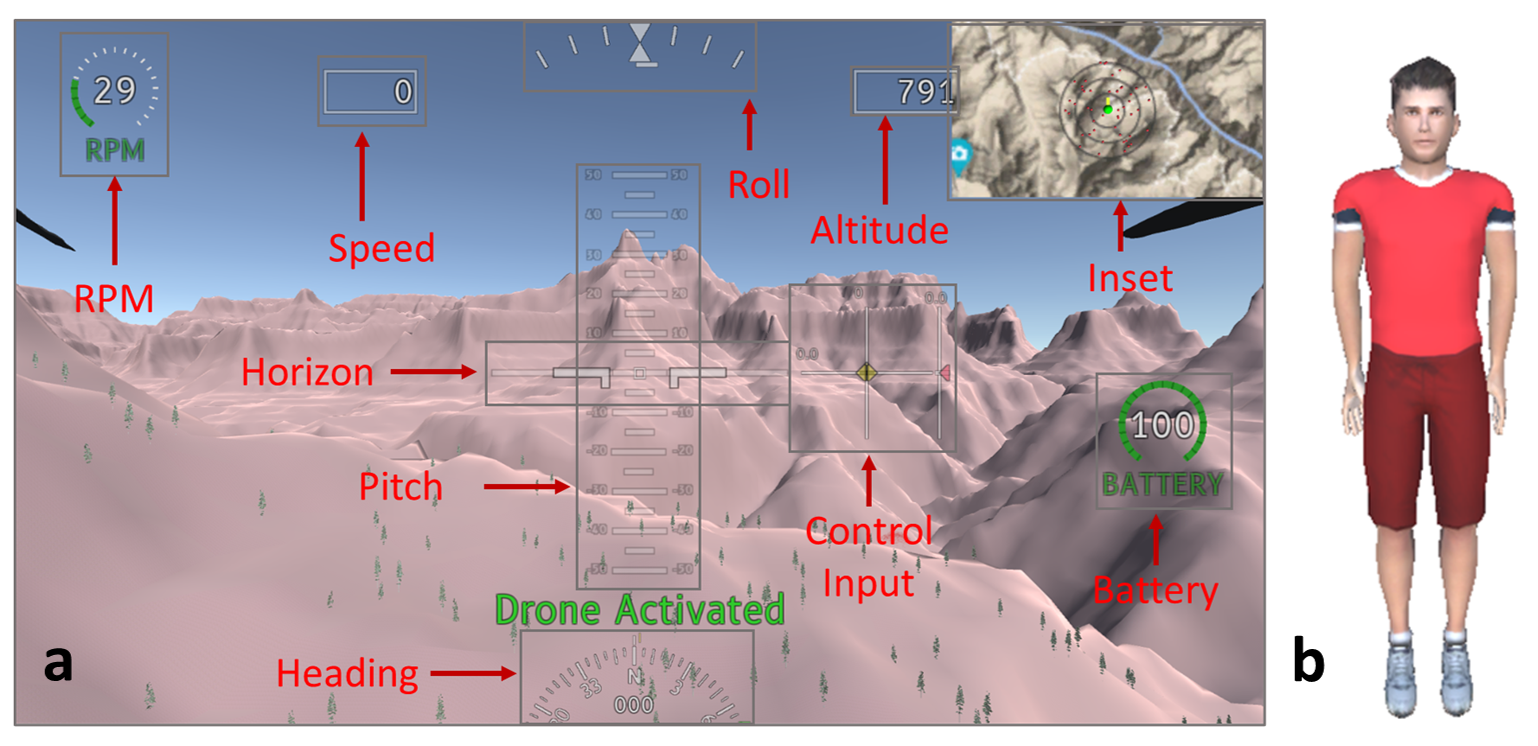
\includegraphics[width=0.99\linewidth]{images/hud.png}
		\caption[width=0.99\linewidth]{ FPV display (a) as seen by the teleoperator. The inset in the top right corner, shows the three POAs in black circles, the position of the teleoperated UAV (filled green circle), and other UAVs (red circles). The missing person (b) was placed within random locations within the virtual environment. See video of a sample search at \url{https://youtu.be/3E6V3mOa7AM} }
		\label{fig:HUDandMissingPerson}
	\end{figure}
	
	\subsection{Experimental Setup} 
	The experimental setup consisted of a desktop computer with a wide-screen monitor (2560 $\times$ 1080 pixels, 60 Hz refresh rate, LG) to present the virtual environment, a fourteen-channel EEG device (Emotiv Epoc X, Emotiv Inc.) sampling at 256Hz to record brain activity, and an eye tracking device recording gaze position at 150 Hz (Pupil Core, Pupil Labs inc.). Lab streaming layer was used to record time-synchronized  EEG, gaze, and keypress data. A chin rest was placed on the table at a fixed distance from the monitor to reduce head movement.
	
	\subsection{Experimental Conditions}
	The experimental conditions consisted of varying the type of prior knowledge available and the distribution of the UAV swarm within the environment. Specifically, prior knowledge could be about the missing person in the form of their approximate distance from the PLS (two values, corresponding to whether such information was shown or not), terrain in the form of walking trails (two values, corresponding to whether they were shown or not), and distribution of the UAV swarm (two values, spread out uniformly or clustered on a random location within the outer two POAs; the random location had no relation to the actual location of the missing person). 
	
	Correspondingly, we tested eight conditions, where each condition is encoded as a three-letter acronym depicting the presence of prior knowledge of missing person (Y/N), terrain (Y/N), and the distribution of swarm (U/C). For example, the condition NNU corresponds to where no prior knowledge was given about missing person or the terrain, and the UAV swarm were distributed uniformly through the environment; similarly the condition YYC corresponded to the prior knowledge provided for both the missing person and the terrain, and the UAV swarm clustered within the two outer POAs. 
	
	
	
	\subsection{Experimental Procedure}
	
	Twenty participants (16 males and 4 females, aged 24 $\pm$ 4 years) were recruited through flyers and email announcements. Candidates were excluded if they were under 18 years of age, if they wore prescription glasses to prevent potential interference with eye-tracker, or if they had thick scalp hair which could prevent EEG headset from obtaining a reliable connection with the scalp. The experiments performed here were approved by the institutional review board under protocol ID HS23-0233. 
	
	Prior to the experiment, each participant was assigned a random six-digit number and asked to review and sign a consent form. The consent form listed the purpose of the study, potential risks, and the type of data that will be collected (EEG, eye tracking, and survey responses). Participants were then asked to put on the EEG headset using a reference image. The electrodes were then adjusted until a reliable connection was obtained. This was followed by instructions on how to teleoperate the UAV, details and purpose of the search mission, meaning of the POA circles, the different information shown on the FPV display, how to indicate having found the missing person, and how to recover from a crash. A multiple choice questionnaire was then given to the participants to test their understanding. Participants were next asked to put on the eye tracker which was then calibrated.
	
	The experiment began with a familiarization trial followed by eight test trials. Each participant was given a printed briefing prior to every trial including the familiarization trial. The briefing started with a paragraph describing the mission as ``A person has gone missing while hiking the trails of the Grand Canyon...'' and denotes that they were last seen 36 hours ago at a location marked with a dot on a section of the map. The briefing further added that the circles centered at the PLS have radii 0.36 km, 0.72 km, and 1.08 km. Information like UAV battery time and the possibility of seeing emergency flares near the missing person is also provided within the briefing. 
	
	
	
	
	
	
	\begin{figure}[ht!]
		\centering
		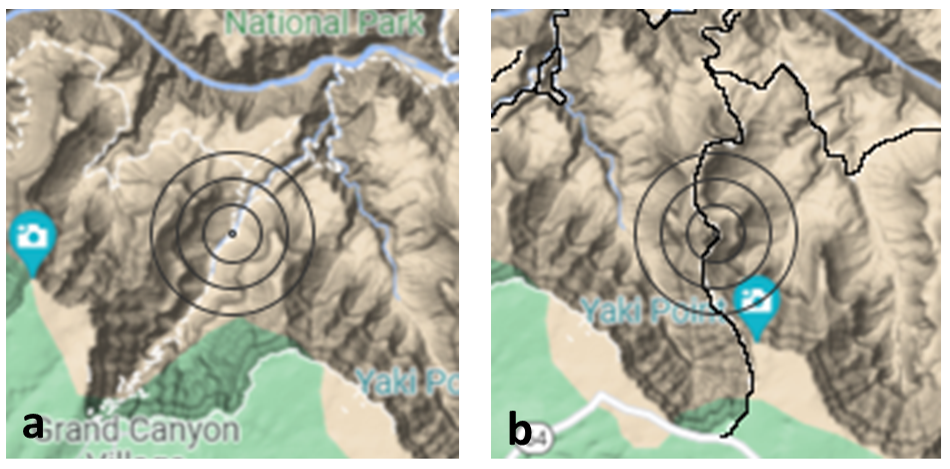
\includegraphics[width=0.5\textwidth]{images/terrainKnowledge.png}
		\caption[width=0.5\textwidth]{Printed maps obtained from an online map with shaded terrain \cite{googlemaps} was provided to the participants as part of their briefings showing the POAs (grey concentric circles), for conditions with no terrain knowledge (a), and with terrain knowledge (b). }
		\label{fig:terrainKnowledge}
	\end{figure}
	
	During the familiarization trial the experimenter helped the participant find the missing person by indicating their precise location on the map on the inset. Post familiarization, the eight conditions were tested in a random order. 
	
	
	During such trials, additional information regarding the missing person and the terrain was provided depending on the condition being tested. Specifically, for missing person*///////////////////////////////////////////////////////////////////////////////////////////////////////////////////////////////////////////////////////////////////////////////////////////////////////////////////////////////////////////////////////////// information the briefing contained italicized text that said ``Based on additional information about the************************************************************************************************************************************************************************************************************************************************************************************************************************************************************************************************************************* person’s physical and mental health, we think that the person may have walked between 0.36 km and 0.72 km (between smallest and the next-sized circle) during the last 36 hours''. For terrain information, the briefing contained text ``Nearby trails are shown in black'' along with trails drawn in black on the printed map within the briefing. Figure \ref{fig:terrainKnowledge} shows the two types of maps provided to participants. The search took place in one of the four locations randomly selected for a condition shown in Figure \ref{fig:grandCanyonTopView}.
	
	
	Trials ended when participants either found the missing person or at approximately 10 minutes when the battery got depleted. Upon finding the missing person, the participant was asked to enter the color of the missing person's t-shirt and pants in a prompt. This was to ensure that the UAV was brought close enough for identification. At the end of every trial, the participant was asked to fill out a NASA-TLX form, which surveyed their mental workload in response to the trial on a 21-point scale. The participants were also offered to take a break after the fourth trial. 
	
	At the end of the experiment, participants were asked to enter their preferred gender and their age, followed by a presence questionnaire which consisted of questions on a 7-point scale. The questions surveyed the participants on their past experience with virtual reality, realism of the environment, responsiveness, where they tended to search for the missing person, and whether the presence of other UAVs affected their search.
	
	
	
	
	\subsection{Data analysis}
	\subsubsection{Calculating cognitive load}
	EEG data was bandpass filtered to keep frequencies between 0.1 and 20 Hz followed by rejection of trials where any of the frontal electrodes posted an absolute amplitude above 1000 $\mu V$ for greater than 5\% of the length of the trial. This led to approximately 6\% of the trials getting rejected.  
	
	Cognitive load was calculated from the filtered data as the degree of reduction in $\alpha$ power denoted by frequencies within the 9.5--11.5 Hz range \cite{arunimCogLoad,Klimesch1999}. Specifically, given an electrode, $k$ the difference between the $\alpha$ power of baseline and trial is $\Delta I^{k}(o) = I_b ^{k} - I_t ^{k}(o)$, where the baseline power $I_b^k$ is measured over data from 5 seconds prior to the start of the trial, and the trial power $I_t^k(o)$ is measured over a variable observation window of length $o$ seconds since the beginning of the trial. Cognitive load is next measured as the weighted average over all the frontal electrodes.
	\begin{equation}
		L(t) = \sum_{k=1}^{14}w_k\Delta I^k(o),
	\end{equation}
	where the weights $w_k$ were determined in a previous experimental study involving object identification and classification \cite{arunimCogLoad}. Any cognitive load value that lied beyond three times the standard deviation from the mean value across all participants was considered an outlier and removed from the dataset.
% \subsubsection{Generalized Linear Models}
% Generalized linear mixed model refers to a linear regression model for a continuous response (focus) variable given some predictors. In GLM, three assumptions \cite{mccullagh2019generalized} are needed to constrict a regression model:(i) Random Component, which is the probability distribution of the response variable, (ii)Systemic component, which assumes a linear underlying combination of predictor variables and, (iii) link function, which specifies the link between random and systemic components. If the response variable is normally distributed, GLM becomes a simple linear regressional problem. 
%A general technique to build GLM model is to add predictor variables stepwise to the general model and check for the goodness of fit. We iteratively develop a model which best describes the response variable (cognitive load). The first step in such a process is to successively add predictor variables' main and interaction effects, and measure each effect's significance.

	
	
%	\subsubsection{Calculating fixation and dwell time}
%	The gaze location output from the eye tracker is in terms of normalized coordinates between 0 and 1, where the extreme values correspond to the lower left corner and upper right corner of the field of view. These values were mapped to computer screen pixel coordinates with a custom application designed in windows presentation software. This application which was run prior to the experiment, asked the participants to fixate at the center of a cross-hair at nine different locations on the display. A second order polynomial is then fit to the normalized coordinates ($x_i,y_i$) at location $i$ to output the pixel coordinates $(X_i,Y_i)$ as
%	
%	\begin{equation}
%		\begin{aligned}
%			X_i =a_0 + a_1 x_i + a_2 x_i ^2 + a_3 x_i y_i \\
%			Y_i = b_0 + b_1 x_i + b_2 x_i ^2 + b_3 x_i y_i,
%		\end{aligned}
%	\end{equation}
%	where, $a_{0,1,2}$ and $b_{0,1,2}$ are constants found by solving the over-determined system of equations.
%	
%	A dispersion-threshold identification (I-DT) algorithm was used to quantify gaze fixation from the calibrated gaze data \cite{salvucci2000identifying}. The I-DT algorithm identifies a group of consecutive gaze points as fixation based on an angular dispersion (how far the gaze moves during a set of consecutive points in time) and a minimum duration (how long the gaze stays within a particular region). In this study, we selected a dispersion threshold of 1$^{\circ}$ and a minimum duration threshold of 200 ms.
%	
%	In our case, the dispersion threshold in degrees was converted to 8.5 mm of arc on the computer monitor using the distance of chin rest from the monitor, which was then used to determine fixation events. In particular, consecutive gaze locations were marked as fixation events if the traverse distance was less than the dispersion threshold, and cumulative time exceeded the minimum duration threshold. The output of the algorithm was individual fixation event duration and its mean location. This was used to then calculate dwell time defined as the fraction of duration of the fixation events inside an area of interest (AOI) over the duration of the full experiment. In this study the AOI was the inset in the display, selected to analyze how often participants referred to the overhead GPS view during various conditions.
	
\subsubsection{Speed and turn rate}
Trajectory data from the experiments was smoothed with a moving window average of 0.5 seconds and used to calculate speed and turn rate of the UAV. Specifically, given the position $\mathbf{r}(k) \in \mathbb{R}^3$ of the UAV at $k^{th}$ time step, the instantaneous velocity of the UAV was calculated as $\mathbf{v}(k) =\frac{\mathbf{r}(k)-\mathbf{r}(k)}{t(k)-t(k-1)}$ where $t(k)$ is the corresponding timestamp. Given the two-dimensional heading $\theta(k) \in\mathbb{R}$ of the UAV at $k^{th}$ time step, the instantaneous turn rate was calculated as $\omega(k) =\frac{\theta(k)-\theta(k-1)}{t(k)-t(k-1)}$.
	
Statistical analysis was performed by fitting generalized linear mixed models (GLMM) to determine the dependence of different factors on performance, workload, cognitive load, and dwell time percentage. A significant effect was considered if the $p$ value was less than 0.05. If found significant, the value of the estimate of slope compared to range was then noted to comment on the size of the effect. The main effects tested for each of the factors are swarm distribution, missing person knowledge, and terrain knowledge. For cognitive load, length of observation window was also tested for main effect along with interaction effects with missing person and terrain knowledge. 
	%\vspace*{-5cm}
\clearpage
\section{Results} \label{sec:results}
	%\vspace*{-0.5cm}
	
	% Table generated by Excel2LaTeX from sheet 'Presence'
	\begin{table}[h!]
		\centering
		\caption{Participant response to post experiment questionnaire.}
		\begin{tabular}{|c||c|}
			\multicolumn{1}{c}{\textbf{Questions about Virtual Reality (0-6)}} & \multicolumn{1}{c}{Response (mean $\pm$ std)} \\ \hline \hline
			How would you describe your past experience with VR? (rare - frequent) & 1.70  $\pm$ 1.42 \\ \hline
			How responsive did you find the virtual environment? (not responsive - very responsive) & 3.40  $\pm$ 1.19 \\ \hline
			How comfortable did you feel? (very uncomfortable - very comfortable) & 3.80  $\pm$ 1.54 \\ \hline
			How interested were you to explore the virtual environment? (not interested - very interested) & 3.80  $\pm$ 1.47 \\ 
			\hline
			
			\multicolumn{1}{c}{\textbf{Questions about operating the UAV (0-6)}} &       \\ \hline
			How natural did you find the movement of the quad-rotor (UAV)? (artificial - natural) & 3.30  $\pm$ 1.63 \\  \hline
			How well could you fly through the environment? (with difficulty - with ease) & 4.00  $\pm$ 1.17 \\ \hline
			The extent to which you felt as if you were moving when standing still? (not at all - very much) & 1.95  $\pm$ 1.70 \\ \hline
			Did the presence of other UAVs affect your search? (did not - affected significantly) & 1.10  $\pm$ 1.60 \\ \hline
			
		\end{tabular}%
		\label{tab:presenceQuestionnaire}%
	\end{table}%
	
	\begin{figure*}[htpb]
		\centering
		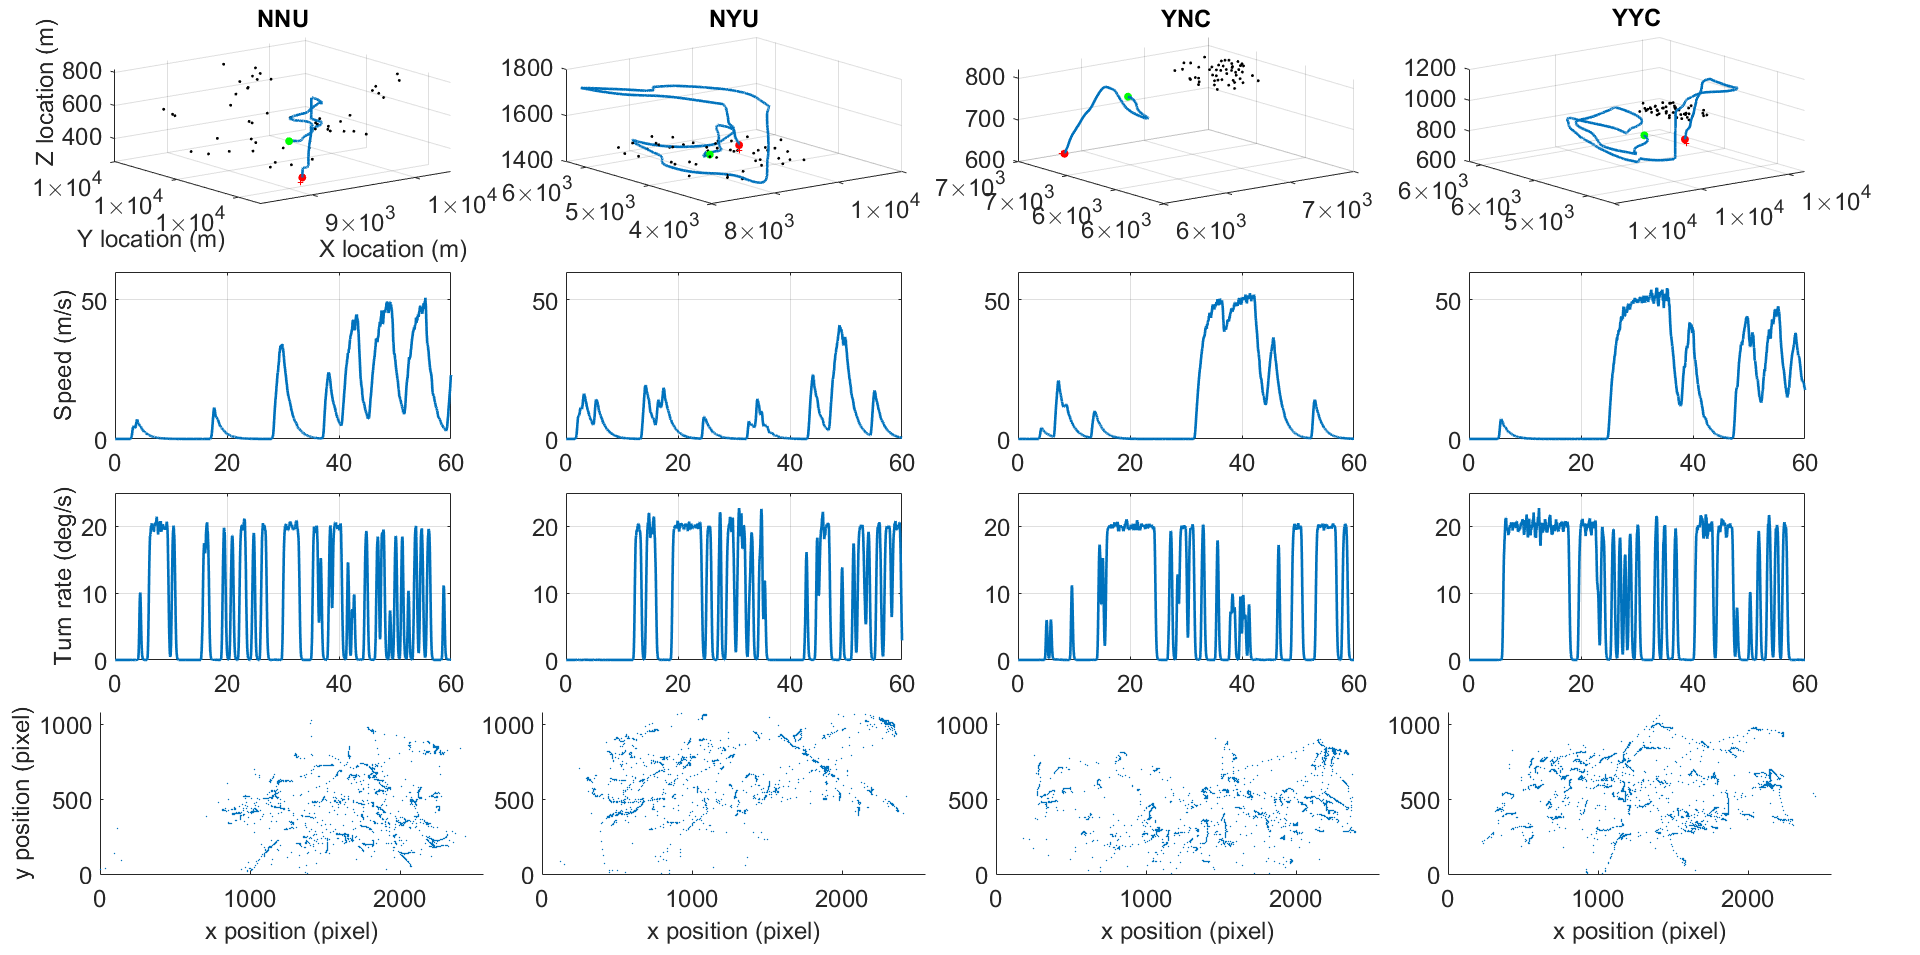
\includegraphics[width=1\textwidth]{images/multiPlot.png}
		\caption[width=0.5\textwidth]{Sample data of a single participant showing the trajectory of the teleoperated UAV (top row), speed of the UAV (second row from top) turn rate (third row from top) and shows the gaze of the participant on the display (bottom row). Trajectory is shown for the full length of the experiment, whereas speed, turn rate, and gaze are shown for the first sixty seconds only.}
		\label{fig:multiplot}
	\end{figure*}
	
	\begin{table}
		\centering
		\caption{GLMM estimates of mission performance, cognitive load, dwell time, and UAV movement as a function of various independent factors.  Values in bold indicate significant factors.}
		\begin{tabular}{|c|c|c|}
			%\centering
			
			%\begin{tabular}{|p{1.8in}|c|c|}
			\hline
			\textbf{Predictor (min, max value)} & \textbf{Estimate} & \textbf{p} \\ \hline 
			
			\multicolumn{3}{|c|}{\textbf{Performance} (0,600 seconds)} \\ \hline 
			Intercept & 285.468 & $<$ 0.001 \\ \hline
			
			Swarm distr (U,C) & -90.931 & \textbf{0.001} \\ \hline
			
			Prior knowledge, missing person (N,Y)    & -66.66 & $<$ \textbf{0.016} \\ \hline
			Prior knowledge, terrain (N,Y) & 2.818 & 0.917 \\ \hline 
			
			\multicolumn{3}{|c|}{\textbf{Average Speed} (0, 50 m/s)} \\ \hline 
			
			Intercept & 27.405 & $<$ 0.001 \\ \hline
			
			Swarm distr (U,C) & -3.152 & \textbf{0.0293} \\ \hline
			
			Prior knowledge, missing person (N,Y)  & -1.488 &  0.303 \\ \hline
			
			Prior knowledge, terrain (N,Y)) & 1.461 & 0.3031 \\ \hline
			
			\multicolumn{3}{|c|}{ \textbf{Average Turn Rate} (0, 25 $^\circ$/s)}  \\ \hline 
			Intercept & 6.165 & $<$ 0.001 \\ \hline
			
			Swarm distr (U,C) & -0.555 & 0.174 \\ \hline
			
			Prior knowledge, missing person (N,Y)    & -0.864 &  \textbf{0.036} \\ \hline
			
			Prior knowledge, terrain (N,Y) & -0.262 & 0.519 \\ \hline 
			
			\multicolumn{3}{|c|} {\textbf{Cognitive Load} (-4.785, 3.749 $\mu V^2/Hz$)} \\ \hline 
			Intercept & -0.706 & $<$0.001 \\ \hline
			
			Swarm distr (U,C) & -0.089 & $<$ \textbf{0.002} \\ \hline
			
			Prior knowledge, missing person (N,Y) & -0.016  & 0.781 \\ \hline
			
			Prior knowledge, terrain (N,Y) & 0.142  & \textbf{0.017} \\ \hline
			
			Obs window (1-25 s) & 0.071 & $<$ \textbf{0.001} \\ \hline
			
			Prior knowledge, missing person (N,Y):Obs window (1-25 s) & 0.001 & 0.831 \\ \hline 
			Prior knowledge, terrain (N,Y):Obs window (1-25 s) &-0.011 & \textbf{0.004} \\ \hline 						
			%\end{tabular}%
		\end{tabular}
		\label{tab:allGLMM}%
		
	\end{table}
	\begin{figure}[ht!]
		\centering
		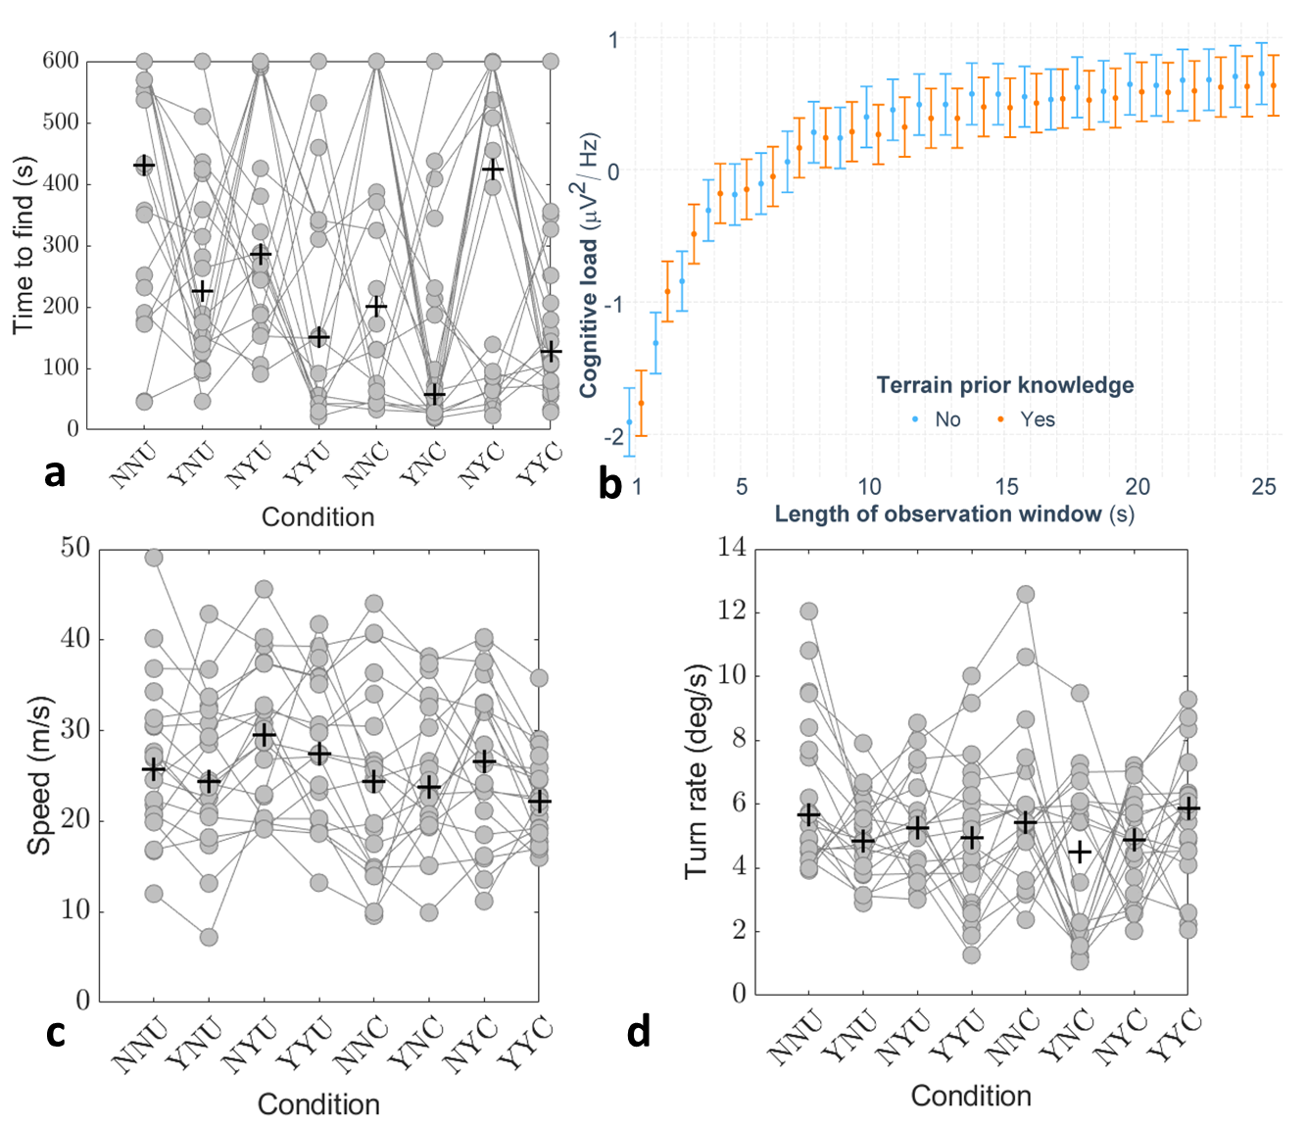
\includegraphics[width=0.99\linewidth]{images/speedTurnPerformanceCogload.png}
		\caption[width=0.99\linewidth]{Average time to find (a) across all conditions. Average cognitive load with and without prior knowledge of terrain (b) across all trials as a function of observation window length. Average UAV speed (c) and turn rate (d) across all conditions. Connected points indicate the same participant and '+' indicates median. }
		\label{fig:speedandTurnRate}
	\end{figure}
	
	
	\subsection{Realism of the virtual environment}
	
	
	Participants responses to questions related to the virtual environment revealed that they found the environment to be responsive and comfortable and that they were generally eager to explore the virtual environment  (Table \ref{tab:presenceQuestionnaire}). In regards to operating the UAV, they found it was controllable and felt the movement to be natural.
	
	\subsection{Sample trajectories}
	
	Figure \ref{fig:multiplot} showcases a single participant's trajectory, speed, turn rate, cognitive load and gaze data for four out of eight trials. In general, we found that participants took about 20 seconds to start flying faster and actively searching. Participant gaze appears clustered either around the top right section of the display, which corresponded to the inset, or near the extreme right which corresponded to the battery level indicator. %Cognitive load is calculated in one second windows for sixty seconds, in this case the cognitive load is negative because it is calculated as the degree of desynchronization in $\alpha$ power band \cite{Klimesch1999}, for the window size used the desynchronization is not significant enough to warrant a positive cognitive load.
	
	
	
	\subsection{Search performance}
	
	
	% Table generated by Excel2LaTeX from sheet 'Performance'
	% \begin{table}[ht!]
		%   \centering
		%   \caption{GLM on showing the main effects of swarm cohesion, prior knowledge of target and mission person on the performance.}
		%     \begin{tabular}{|l|c|c|}
			%      \hline
			%      \textbf{Predictor} & \textbf{Estimate} & \textbf{p} \\ \hline
			%     Intercept & 376.435 & $<$ 0.001 \\ \hline
			%     SwarmCohesion(High) & -75.583 & \textbf{0.019381} \\ \hline
			%     TargetKnowledge(Yes)    & -125.087 & $<$ \textbf{0.001} \\ \hline
			%     TerrainKnowledge(Yes) & 5.092 & 0.873748 \\ \hline
			%     \end{tabular}%
		%   \label{tab:performanceGLM}%
		% \end{table}%
	The GLMM analysis in table \ref{tab:allGLMM} shows that swarm distribution and missing person knowledge significantly affected the performance. Negative values of estimate for the significant factors show that, time to find the missing person reduced when the swarm was clustered within the last two POAs, and when the participant had prior knowledge about the missing person. Figure \ref{fig:multiplot}a shows the search performance, measured in terms of time to find the missing person knowledge, for each condition.
	
	% \begin{figure}[ht!]
		% \centering
		% 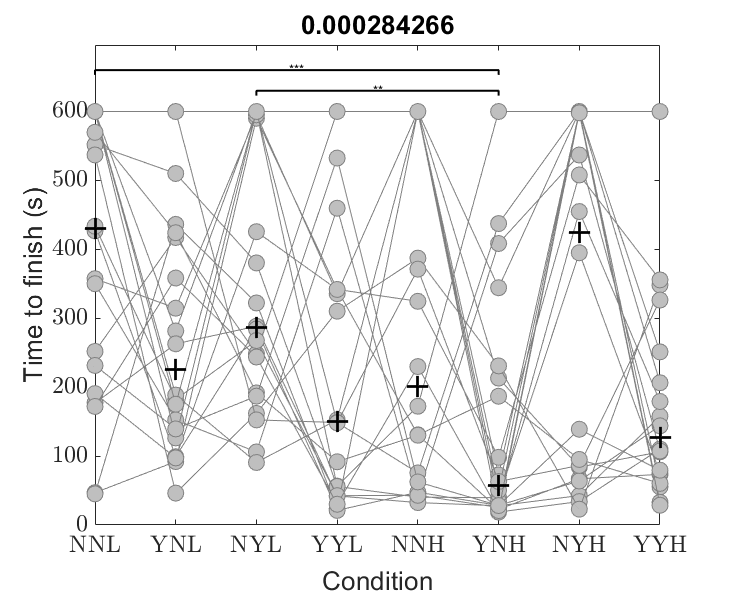
\includegraphics[width=0.4\textwidth]{images/time2finish.png}
		% \caption[width=0.5\textwidth]{Post-hoc result for performance i.e. time taken to complete the mission and showing statistically significant variance between the different conditions.}
		% \label{fig:time2finish}
		% \end{figure}
	
	%This measure also shows that there is significant effect on search performance measured as time to find target in seconds ($\chi^2$(7,20) = 27.38,p $<$ 0.001). 
	
	
	
	\subsection{Cognitive load}
	
	
	
	
	Table \ref{tab:allGLMM} also shows that observation window, swarm distribution and terrain knowledge significantly affect cognitive load. A clustered swarm reduced the cognitive load, whereas increasing observation window size and terrain knowledge resulted in higher cognitive load. The interaction effect between terrain prior knowledge and observation window showed a negative estimate indicating that, when terrain knowledge was available, cognitive load was higher earlier during the experiment (shorter observation window) but then decreased as the experiment progressed. Figure 5b confirms this by showing cognitive load as a function of observation window as it ranged from 1 to 25 seconds for all trials. Here we see that the cognitive load rises initially before leveling off at around 5 seconds.
	
	
	% Table generated by Excel2LaTeX from sheet 'Sheet1'
	
	
	\subsection{NASA-TLX responses}
	% Table generated by Excel2LaTeX from sheet 'Sheet1'
	\begin{table}[H]
		\centering
		\caption{NASA-TLX responses on a 0--20 scale across different conditions}
		\resizebox{1\linewidth}{!}{
			\begin{tabular}{|c|c|c|c|c|c|c|}
				\multicolumn{1}{c}{Condition}  & \multicolumn{1}{c}{Mental} & \multicolumn{1}{c}{Physical} & \multicolumn{1}{c}{Temporal} & \multicolumn{1}{c}{Performance} & \multicolumn{1}{c}{Effort} & \multicolumn{1}{c}{Frustration} \\ \hline \hline
				NNU & 7.3   $\pm$ 5.2   & 3.9   $\pm$ 4.3   & 6.4   $\pm$ 5.4   & 10.2  $\pm$ 7.9   & 9.7   $\pm$ 5.4   & 5.8   $\pm$ 4.4 \\
				YNU & 6.3   $\pm$ 5.4   & 2.8   $\pm$ 4.2   & 5.7   $\pm$ 4.4   & 14.7  $\pm$ 5.5   & 8.1   $\pm$5.5   & 4.5   $\pm$ 3.9 \\
				NYU & 7.0   $\pm$5.4   & 2.7   $\pm$ 3.6   & 6.0  $\pm$ 4.7   & 12.7  $\pm$ 6.6   & 7.7   $\pm$ 5.0   & 5.4   $\pm$ 5.0 \\
				YYU & 5.9   $\pm$ 5.3   & 2.3   $\pm$ 3.4   & 5.1   $\pm$ 5.1   & 14.7  $\pm$ 7.2   & 6.5   $\pm$ 5.9   & 4.0   $\pm$ 5.2 \\
				NNC & 6.9   $\pm$ 6.2   & 2.8   $\pm$ 4.3   & 5.3   $\pm$ 5.6   & 12.2  $\pm$ 8.6   & 6.9   $\pm$ 6.3   & 4.9   $\pm$ 6.0 \\
				YNC & 4.9   $\pm$ 5.9   & 3.4   $\pm$ 5.8   & 3.6   $\pm$ 3.6   & 16.8  $\pm$ 5.4   & 5.2   $\pm$ 5.7   & 3.6   $\pm$ 5.7 \\
				NYC & 6.8   $\pm$ 6.3   & 3.3   $\pm$ 5.1   & 5.4   $\pm$ 5.0   & 11.0  $\pm$ 8.4   & 8.1   $\pm$ 6.0   & 6.5   $\pm$ 6.6 \\
				YYC & 5.1   $\pm$ 4.6   & 2.6   $\pm$ 2.7   & 4.4   $\pm$ 4.2   & 16.0  $\pm$ 5.2   & 6.9   $\pm$ 5.8   & 4.0   $\pm$ 5.8 \\ \hline \hline
			\end{tabular}%
		}
		\label{tab:surveyTLX}%
	\end{table}%
	Table \ref{tab:surveyTLX} shows the average responses to NASA-TLX survey questions posed to participants after every session. Participants felt that they had to work somewhat hard to accomplish the task for conditions where they did not have missing person prior knowledge. The participants also did not find the tasks to be particularly mentally or physically challenging. In general their frustration levels were low and did not feel rushed to finish the task. Participants generally rated their performance as good.
	

\subsection{Search behavior}
	
	
Table \ref{tab:allGLMM} shows that average speed of participant was affected by the swarm distribution, with the negative estimate implying that a clustered swarm led to lower average speeds. Turn rate on the other hand is affected by missing person knowledge with a slightly lower turn rate when missing person knowledge was available. Figures \ref{fig:speedandTurnRate}c and d show the average speed and average turn rate across all conditions.
	


\clearpage

\section{Classifying prior knowledge based on UAV movement} \label{sec:LSTM}
\subsection{LSTM model selection}
We sought to model the human tele-operator's response to  prior knowledge about the terrain and missing person using a long-short-term memory (LSTM) neural network. Specifically, our goal is to infer prior knowledge of the tele-operator based on the movement of the UAV as they searched for the missing person. This inference, which can be made by other autonomous UAVs who can observe the teleoperated UAV, will in turn be used to control their swarming behavior. A trained LSTM neural network model will be used to constantly monitor the movement of the teleoperated robot and will provide prior knowledge of the teleoperator in real-time. 
\textit{$<$need to justify observation time$>$}

To train the model, speed and turn rate data was partitioned into $T-second$ segments and input to the LS-TM model whose output was the probability of a particular type of prior knowledge (missing person knowledge or terrain knowledge). The swarm cohesion was not considered as a factor in the participant's decision making as the post experiment survey showed that the participants tended to ignore the swarm clusters after the first few tries. Accuracy of the model was calculated as the highest average accuracy for a test data set for any parameter set. 

We use multi-label classification to gauge the knowledge of the operator. A three letter word in the form $XYZ$ is used to define prior knowledge of the missing person (yes Y, no N), prior knowledge of the terrain (yes Y, no N) and, swarm cohesion level (high H, low L), where each of the letters in $XYZ$ is replace by corresponding knowledge level. Since, swarm cohesion is being ignored by the participants, all the trainable dataset was collapsed into $XY$ form. The multi-label classification directly provides the amount of prior knowledge a person possesses in each of the 2 categories. The neural network was trained on over 12 hours of trajectory data, generated by the participants in course of the experiment.

%<what are the labels, what probabilities were assigned, how much data was used>.

The initial model of the neural network was based on \cite{karim2018lstm} which has been shown to work well for time-series classification. The original model was adapted to enable two input features and instead of multi-class classification, a multi-label classification was used. To optimize the model, we used a variation of k-fold cross validation to find the optimal hyper parameters as described in table \ref{alg:KFold}. The hyper parameters tested for training the neural network are mini-batch size and the observation time. Figure \ref{fig:NNarchitecture}, shows the neural network architecture used in this study.


\begin{figure}[ht!]
\centering
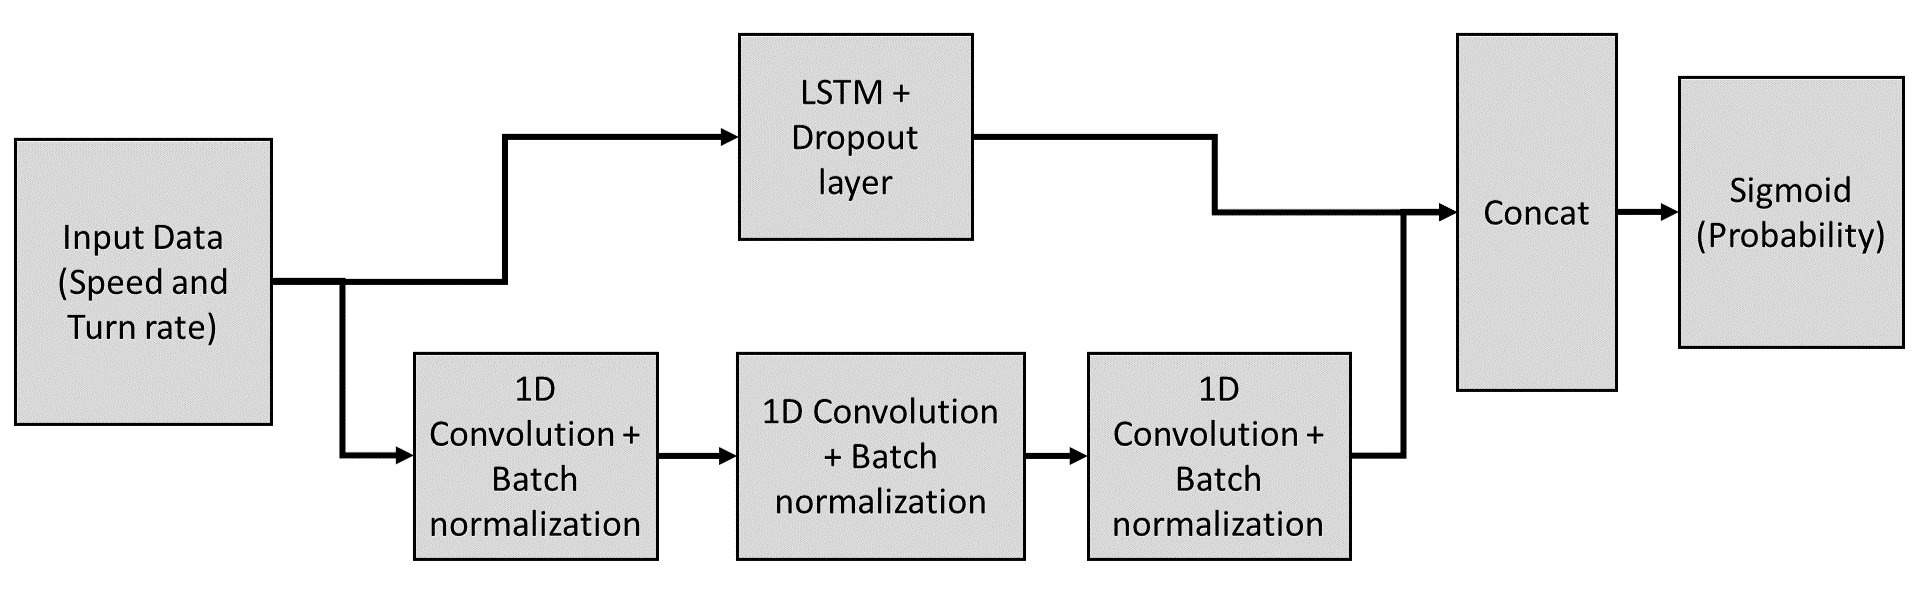
\includegraphics[width=0.8\textwidth]{images/LSTM_pictorial.png}
\caption[width=0.5\textwidth]{The neural network architecture as used in this paper. }
\label{fig:NNarchitecture}
\end{figure}


\begin{algorithm}
\caption{k-Fold algorithm to obtain optimal parameter set for LSTM training.}\label{alg:KFold}
Dataset $D$, $K_1$ outer iterations, $K_2$ inner iterations and, $P$ parameter sets.
\begin{algorithmic}
\For{i = 1 to $K_1$}
    
    \State randomize $D$ dataset by subjects
    \State $train_1 \gets $ 80\% of randomized dataset
     \State $test_1 \gets $ 20\% of randomized dataset
    \For{j = 1 to $K_2$}
        \State randomize $train_1$ dataset by subjects
        \State $train_2 \gets $ 80\% of $train_1$ dataset
        \State $test_2 \gets $ 20\% of $test_1$ dataset
        \For{each $p$ in $P$ parameter set}
            \State $M2 \gets$ create model with $p$ parameters
            \State train $M2$ with $train_2$ dataset
            \State validate $M2$ with $test_2$ dataset
        \EndFor
    \EndFor
    \State Select the hyper parameter set $p$ with highest validation accuracy
    \State $M1 \gets$ create model with selected hyper parameters
    \State train $M1$ with $train_1$ dataset
    \State validate $M1$ with $test_1$ dataset
\EndFor

\State Select hyper-parameters with highest averaged maximum accuracy over parameter sets
\end{algorithmic}
\end{algorithm}


%<details about the k-fold validation that was performed to optimize the number of nodes, number of layers, epochs> 

\clearpage
\subsection{Observation time selection}
Observation time is the duration for which the tele-operated robot must be tracked by an autonomous UAV swarm in order to make an accurate inference of the prior knowledge. To select an observation time we ran the model with optimal hyper-parameters for different time segments using a K-fold cross validation, then averaged the maximum accuracy for every parameter set. From fig. \ref{fig:AvgMaxAcc}, observation time of 15 seconds shows average accuracy of $0.7 \pm 0.07$, which is optimal for our purpose.

\begin{figure}[ht!]
\centering
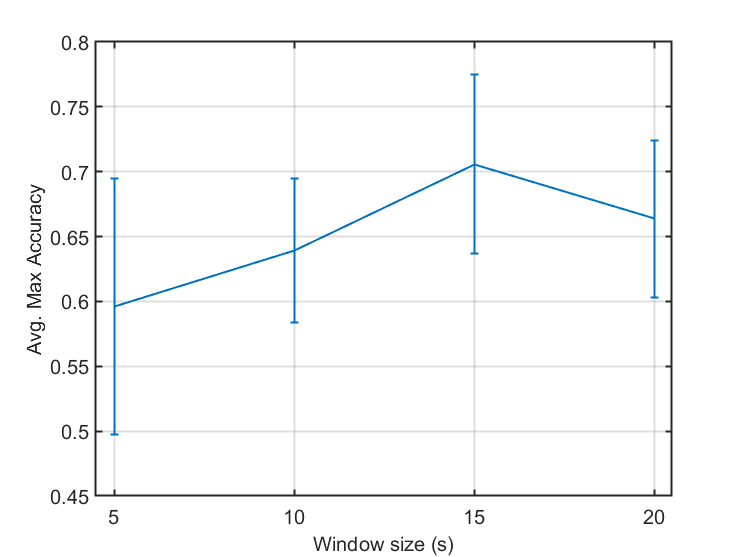
\includegraphics[width=0.7\textwidth]{images/maxAccuracyResults.png}
\caption[width=0.5\textwidth]{Average maximum accuracy plots.}
\label{fig:AvgMaxAcc}
\end{figure}


%<show figure and discuss>
\section{Swarm response to prior knowledge inference}
\subsection{Control strategy} \label{sec:controlStrategy}
In this section we formulate and compare a closed loop control strategy of an autonomous swarm using prior knowledge of the human operator to accelerate the search for missing person. Specifically, we replay the experimental trajectory in the presence of a swarm that a) acts on prior knowledge based closed loop control strategy, b) blindly follows the human as a leader, c) a random search model. In addition, we also have the swarm follow and ignore a simulated teleoperator that follows a spiral trajectory. All of the above swarm strategies operate according to a modified self-propelled particle model called the zonal model \cite{Couzin}. 

The number of agents in the robot swarm is $n-1$, the $n-$th agent is the human operated UAV. The position and velocity of $i-$th agent at time $t$ is given by $\textbf{r}_i(t)\in \mathbb{R}^3$ and $\textbf{v}_i(t) \in \mathbb{R}^3$ respectively. The velocity of the $i-$th agent is updated as,

\begin{equation}
    \textbf{v}_{i}(t+\delta{t}) = \left\{\begin{matrix}
-s_i\mathbf{d}_{i,zor}(t)   \text{ if } \textit{$zor_i$} \neq \emptyset\\
 0.5s_i \left((\mathbf{d}_{i,zoo}(t) + \mathbf{d}_{i,zoa}(t))(1-k_h) + k_h\mathbf{d}_{i,n}\right)
\text{ otherwise},
\end{matrix}\right.
\label{eq:zonalModel}
\end{equation}

where,$\mathbf{d}_{i,zor}=\sum_j\frac{\mathbf{r}_i-\mathbf{r}_j}{|\mathbf{r}_i-\mathbf{r}_j|}$, $\mathbf{d}_{i,zoo}=\sum_j\frac{\mathbf{v}_j}{|\mathbf{v}_j|}$, 
and $\mathbf{d}_{i,zoa} = -\mathbf{d}_{i,zor}$ and $\mathbf{d}_{i,n}= \frac{\mathbf{r}_n-\mathbf{r}_i}{|\mathbf{r}_n-\mathbf{r}_i|}$; $i$ and $j$ represent focal agent and neighboring agent respectively ($i \neq j$), $n$ is the subscript for the human participant, and $\delta t$ denotes the simulation time step in seconds; $s_i \in \mathbb{R}$ denotes constant speed. Model parameters $zoo$, $zor$, and $zoa$, can be varied to produce different types of behavior \cite{Couzin}.

%This updated model has two distinct parameters that directly determine the interaction of the swarm with the human participant. First, the value of $zor$ which determines how far spread out the swarm can be (e.g. clustered versus near uniform) and second the gain $k_h$ which determines how close the swarm will get to the human teleoperator. With respect to $zor$ if the teleoperator has person or terrain knowledge, we design the swarm strategy to remain close to the teleoperator, therefore, 
%
%\begin{equation}
%    \textbf{zor}_{i}(t) = \left\{\begin{matrix} r_{fov} & \text{ if random search} \\
%    r_{fov} & \text{ if follow operator}\\
%    r_{fov}(1+P_K(t))  &\text{ otherwise},
%\end{matrix}\right.
%\label{eq:zonalModel1}
%\end{equation}
%
%where $zor=r_{fov}$ enables no overlap of field of views ensuring that maximum coverage is attained.

This updated model has the gain $k_h$ which determines how close the swarm will get to the human teleoperator. 
The missing person and terrain knowledge are denoted by $P_K(t)$ and, $T_K(t)$ respectively, the detection radius $r_{fov}$ ($=100 m$) and, $k_h(t)$ gain is used to modify the behavior so that both the probability of terrain or missing person is treated equally as:
\begin{equation}
    \textbf{k}_{h}(t) = \left\{\begin{matrix} 0.0 & \text{ if random search} \\
    1 & \text{ if follow operator}\\
    0.5(T_K(t)+P_K(t))  & \text{ otherwise},
\end{matrix}\right.
\label{eq:zonalModel2}
\end{equation}

\begin{table}[htbp]
  \centering
  \caption{Control Loop strategies in extreme cases of prior knowledge.}
    \resizebox{0.8\linewidth}{!}{ \begin{tabular}{|c|c|c|c|}
    \hline
    $P_K$ & $T_K$ & Action & Justification \\
    \hline
    1     & 0     & Large separation of swarm, strong following & Increased coverage over the same terrain \\
    \hline
    0     & 1     & Low swarm separation and strong following & Strong overlap in the same terrain because terrain knowledge. \\
    \hline
    1     & 1     & Large separation, very strong following & Increased coverage in the same terrain \\
    \hline
    0     & 0     & Small separation, weak following & Not trusting the human operator, swarm searches randomly \\
    \hline
    \end{tabular}%
    }
  \label{tab:extremePriorKnowledge}%
\end{table}%
In case of the closed loop control strategy, the action of the swarm is under absolute condition i.e. when the probabilities of the available prior knowledge is either 0 or 1 are summarized in table \ref{tab:extremePriorKnowledge}. If the human operated UAV has no knowledge about the terrain or the missing person, the swarm searches randomly and doesn't trust the human at all, if only missing person knowledge is available there would be large separation between the UAVs and the swarm would somewhat follow the human, in case where both the knowledge are available, the swarm completely trusts the human and would follow the human strongly with large separation.

%<formally state it start by coping from the document>
\subsection{Simulation setup}

\begin{figure}[ht!]
\centering
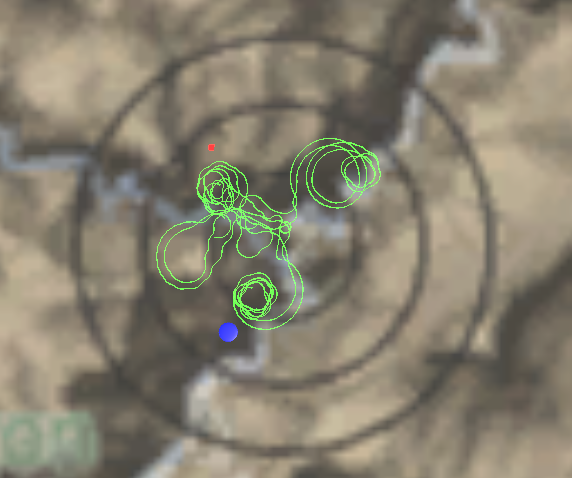
\includegraphics[width=0.5\textwidth]{images/playBackScreenShot.png}
\caption[width=0.5\textwidth]{Instance of a random search simulation, green dots show swarm robots, red dot shows position of the human operated robot and the blue disc shows the location of the missing person.}
\label{fig:playBackSim}
\end{figure}

In order to test the different search strategies, a simulation which plays back the trajectory of the participant is setup. In the original experiment, the swarm of autonomous robots were either clustered in a random location or spread out uniformly over the search area, however in the simulation the swarm exhibit different behaviors depending on the search strategy. The closed loop control strategy uses a neural network trained in python using tensorflow module exported for C$\#$.

A dedicated environment was setup in unity for the simulation, the terrain is identical to the one used in the experiment. This environment plays back the participants' recorded trajectory, however it is interpolated with a time step of 0.04 $s$. A swarm of autonomous UAV is initialized at the location of the person last seen. Figure \ref{fig:playBackSim} shows the top view of the simulation environment with position last seen (PLS) represented by a black dot and probability of area (POA) shown in grey circles are projected on the map. In our case we set the value of $zor = r_{fov}$ and $zoo = zor + 8$ and $zoa = zoo + 14$ to correspond with the dynamic parallel behavior in \cite{Couzin}. 


Figure \ref{fig:playBackSim}, shows instance of a random search strategy by a swarm of 5 robots, the human operated robot trajectory is played back as recorded during the experiment. The swarm behavior is coded differently for different search strategy, a) human operated UAV follows a spiral pattern with a width of $r_{fov}$ with the same speed as that of the average speed of the participants in the experiment as the rest of the swarm follows the human with $k_h=1$ and matching its speed with the teleoperator, b) human operated UAV follows a spiral pattern with the same speed as that of the average speed of the participants in the experiment as the rest of the swarm with $k_h=0$ with the average human speed, c) swarm ignores the human operated UAV  in case of random search with the average human speed, d) swarm follows the human in case of follow search matching the human speed, e) swarm operates on a control strategy as described in section \ref{sec:controlStrategy} matching the human speed.

The swarm robots are positioned at approximately 170 $m$ above the lowest elevation of the map, with a field of view of about 30$^{\circ}$, each robot of the swarm can sense presence of the missing person within a 100 $m$ radius directly below it. Every robot in the swarm travels at a constant speed of 50 $m/s$. All search strategies were tested for 5, 10 and 20 swarm size.

Each experimental condition was simulated once, thus providing 160 instances (8 conditions $\times$ 20 subjects) of search for every swarm size. The criteria for a successful swarm search is: a) the missing person was found with a probability of detection of 0.66 and, b) swarm found the missing person 15 seconds prior to the end time recorded for the condition. 
% Whenever the missing person is within the r_fov, generate a random number between 0 and 1 if that number is less than 0.66 detect, otherwise keep generating as long as the person is in r_fov

%<how many simulations, swarm size, terrain is same, height of swarm, field of view, detection criteria>
%<Three strategies>
\section{Results}
The GLMM analysis in table \ref{tab:allGLMM} shows that swarm distribution and missing person knowledge significantly affected the performance. Negative values of estimate for the significant factors show that, time to find the missing person reduced when the swarm was clustered within the last two POAs, and when the participant had prior knowledge about the missing person. Figure \ref{fig:multiplot}a shows the search performance, measured in terms of time to find the missing person knowledge, for each condition.

% \begin{figure}[ht!]
	% \centering
	% 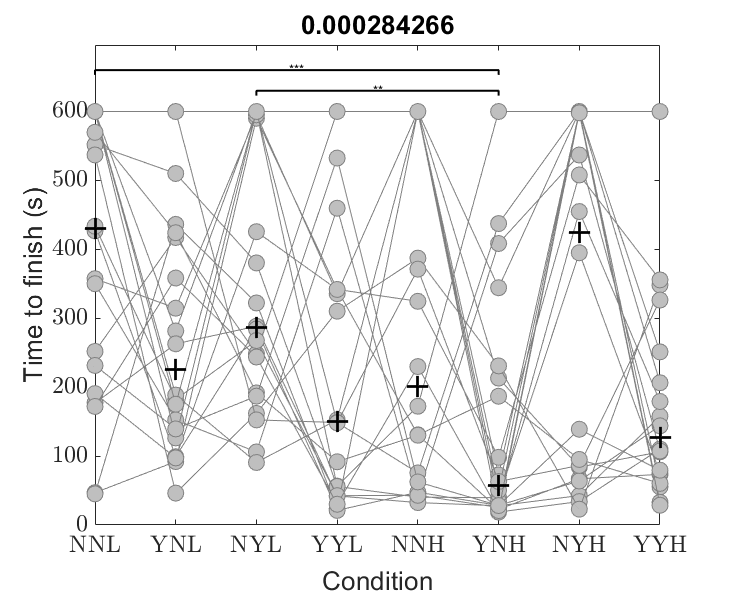
\includegraphics[width=0.4\textwidth]{images/time2finish.png}
	% \caption[width=0.5\textwidth]{Post-hoc result for performance i.e. time taken to complete the mission and showing statistically significant variance between the different conditions.}
	% \label{fig:time2finish}
	% \end{figure}

%This measure also shows that there is significant effect on search performance measured as time to find target in seconds ($\chi^2$(7,20) = 27.38,p $<$ 0.001). 



\subsection{Cognitive load}




Table \ref{tab:allGLMM} also shows that observation window, swarm distribution and terrain knowledge significantly affect cognitive load. A clustered swarm reduced the cognitive load, whereas increasing observation window size and terrain knowledge resulted in higher cognitive load. The interaction effect between terrain prior knowledge and observation window showed a negative estimate indicating that, when terrain knowledge was available, cognitive load was higher earlier during the experiment (shorter observation window) but then decreased as the experiment progressed. Figure 5b confirms this by showing cognitive load as a function of observation window as it ranged from 1 to 25 seconds for all trials. Here we see that the cognitive load rises initially before leveling off at around 5 seconds.


% Table generated by Excel2LaTeX from sheet 'Sheet1'


\subsection{NASA-TLX responses}
% Table generated by Excel2LaTeX from sheet 'Sheet1'
\begin{table}[H]
	\centering
	\caption{NASA-TLX responses on a 0--20 scale across different conditions}
	\resizebox{1\linewidth}{!}{
		\begin{tabular}{|c|c|c|c|c|c|c|}
			\multicolumn{1}{c}{Condition}  & \multicolumn{1}{c}{Mental} & \multicolumn{1}{c}{Physical} & \multicolumn{1}{c}{Temporal} & \multicolumn{1}{c}{Performance} & \multicolumn{1}{c}{Effort} & \multicolumn{1}{c}{Frustration} \\ \hline \hline
			NNU & 7.3   $\pm$ 5.2   & 3.9   $\pm$ 4.3   & 6.4   $\pm$ 5.4   & 10.2  $\pm$ 7.9   & 9.7   $\pm$ 5.4   & 5.8   $\pm$ 4.4 \\
			YNU & 6.3   $\pm$ 5.4   & 2.8   $\pm$ 4.2   & 5.7   $\pm$ 4.4   & 14.7  $\pm$ 5.5   & 8.1   $\pm$5.5   & 4.5   $\pm$ 3.9 \\
			NYU & 7.0   $\pm$5.4   & 2.7   $\pm$ 3.6   & 6.0  $\pm$ 4.7   & 12.7  $\pm$ 6.6   & 7.7   $\pm$ 5.0   & 5.4   $\pm$ 5.0 \\
			YYU & 5.9   $\pm$ 5.3   & 2.3   $\pm$ 3.4   & 5.1   $\pm$ 5.1   & 14.7  $\pm$ 7.2   & 6.5   $\pm$ 5.9   & 4.0   $\pm$ 5.2 \\
			NNC & 6.9   $\pm$ 6.2   & 2.8   $\pm$ 4.3   & 5.3   $\pm$ 5.6   & 12.2  $\pm$ 8.6   & 6.9   $\pm$ 6.3   & 4.9   $\pm$ 6.0 \\
			YNC & 4.9   $\pm$ 5.9   & 3.4   $\pm$ 5.8   & 3.6   $\pm$ 3.6   & 16.8  $\pm$ 5.4   & 5.2   $\pm$ 5.7   & 3.6   $\pm$ 5.7 \\
			NYC & 6.8   $\pm$ 6.3   & 3.3   $\pm$ 5.1   & 5.4   $\pm$ 5.0   & 11.0  $\pm$ 8.4   & 8.1   $\pm$ 6.0   & 6.5   $\pm$ 6.6 \\
			YYC & 5.1   $\pm$ 4.6   & 2.6   $\pm$ 2.7   & 4.4   $\pm$ 4.2   & 16.0  $\pm$ 5.2   & 6.9   $\pm$ 5.8   & 4.0   $\pm$ 5.8 \\ \hline \hline
		\end{tabular}%
	}
	\label{tab:surveyTLX}%
\end{table}%
Table \ref{tab:surveyTLX} shows the average responses to NASA-TLX survey questions posed to participants after every session. Participants felt that they had to work somewhat hard to accomplish the task for conditions where they did not have missing person prior knowledge. The participants also did not find the tasks to be particularly mentally or physically challenging. In general their frustration levels were low and did not feel rushed to finish the task. Participants generally rated their performance as good.

% Friedman repeated measure test shows significant results for participant response to questions on performance and effort. With presence of prior knowledge of the target and terrain (2 levels: Yes, No) revealed that there is a significant effect on performance response ($\chi^2$(7,20) =19.05,p = 0.008) and effort response ($\chi^2$(7,20) = 17.45,p = 0.015). 

% \begin{figure*}[ht!]
	% \centering
	% 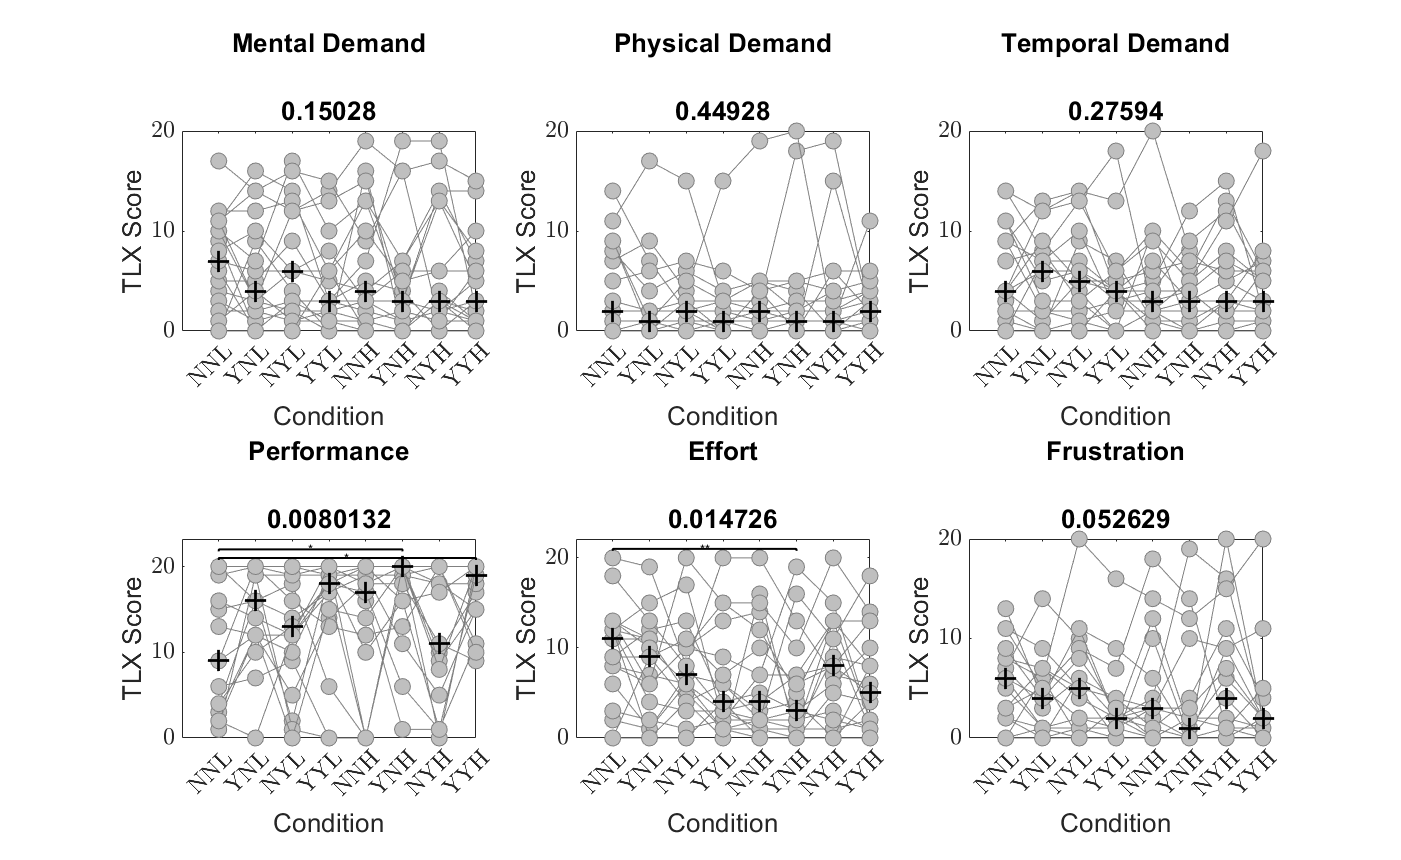
\includegraphics[width=0.8\textwidth]{images/NASA_TLX.png}
	% \caption[width=0.7\textwidth]{NASA-TLX post-hoc results. }
	% \label{fig:NASA_TLX}
	% \end{figure*}
\subsection{Search behavior}


Table \ref{tab:allGLMM} shows that average speed of participant was marginally affected by the swarm distribution, with the negative estimate implying that a clustered swarm led to lower average speeds. Turn rate on the other hand is affected by missing person knowledge with a slightly lower turn rate when missing person knowledge was available. Figures \ref{fig:speedandTurnRate}c and d show the average speed and average turn rate across all conditions.

\subsection{Gaze}
With respect to fraction of dwell time in the inset, we find that terrain knowledge has a significant effect. In particular, if the participant possessed terrain knowledge, they spent significantly more time looking at the inset.




\section{Discussion} \label{sec:discussion}
%<Figure showing fraction of time the swarm found the target before the human. x axis has strategies and y axis has fraction of time>
%<Side by side with another figure showing the time gained (mean+std) for the trials where swarm found the target first. x axis has strategies and y axis has mean +/- std. for example if the swarm finds the target in 4 out of 10 trials, then calculate the difference between time to find by participant (-10 seconds) and the swarm find time.>


Executing a SAR mission with a teleoperated UAV involves taking multiple time-critical decisions. In such a scenario, prior knowledge about the mission would admittedly play an important role. Quantifying this effect on performance, mental workload, and behavior has implications in shared autonomy and user interface design. Furthermore, the perception of other UAVs in the region may influence the actions and in turn performance of the teleoperator. This study was designed to isolate these effects by artificially creating prior knowledge in the form of pre-trial briefings and placing a swarm of UAVs in different spatial distributions. Our results point to several significant effects of prior knowledge and swarm perception on performance, cognitive load, perception and behavior.
	
In terms of workload as measured using NASA-TLX, the tasks were not perceived to be physically demanding, however the participants felt they had to put considerable effort to accomplish the tasks. Low frustration levels indicate that the experiment design was not a significant barrier to accomplishing the task, further supported by the favorable responses regarding the virtual environment and the teleoperation of the UAV.

%in the presence questionnaire. The participants also felts that the UAV was very responsive to commands, which would further reduce the frustration levels, in situations where there is significant latency involved between input and response, the participants would have expressed frustration \cite{khasawneh2019human}.

Mission performance was strongly influenced by the presence of swarm in a cluster and missing person knowledge. It is possible that although the UAV swarm was not necessarily located near the missing person, having it at the same approximate distance from the PLS enabled the participants to waste less time searching within the smaller POA where the missing person was never actually located. Terrain knowledge did not lower the time to find, likely because there were multiple trails for each location, not available on the inset, so that participants may have lost precious time investigating these areas between the display and the printed briefing. Indeed, participants spent more time fixating on the inset when terrain knowledge was available.

Cognitive load was influenced by presence of swarm in the environment, particularly presence of clustered swarm has a negative influence on the cognitive load. A clustered swarm likely provides the participant with an initial direction to search for the missing person, which is probably why cognitive load is low during the first few seconds of the start of the experiment for clustered swarm condition. Terrain knowledge lead to higher cognitive load, which could be because the participants were trying to locate the trails shown to them in the briefings. We also note that the negative value of calculated cognitive load is likely due to the short baseline duration of 5 seconds. In particular future experiments should be planned with a longer rest time for the participants prior to the experiment to ensure that all of the experimental time results in positive cognitive load.   

%The strong coupling between the target knowledge and cognitive load is maybe due to the briefing stating how far the target has moved from PLS, and there are POAs shown in the mini-map on the display. In case of terrain knowledge, the trails are shown only during briefing and not in the mini-map, the participants probably try to look for the trails, however give up when unsuccessful thus we see a weaker coupling.



Ongoing extensions of this work involve controlling an autonomous swarm of robots to assist the teleoperator in their search based on prior knowledge inference. Other applications include shared autonomy where a partially autonomous teleoperated UAV can selectively take over depending on the mental workload experienced by the operator or based on their fixation on a particular location of the environment. Results from this work can also inform intelligent user interfaces that can adaptively display information based on operator attention and cognitive load.
	
	\section{Acknowledgments}
	This research was supported by National Science Foundation under grant \# IIS-2033918.
	%and by Illinois Indiana Sea Grant (IISG) through a graduate student scholars program in 2021-22.


\bibliographystyle{unsrt}
\bibliography{ref.bib}
\end{document}
